\documentclass{article}
\usepackage[utf8]{inputenc}
\usepackage{lineno}
\usepackage{color}
\usepackage{amssymb}
\usepackage{mathtools}
\usepackage{amsthm}
\usepackage{amsmath}
\usepackage{amsfonts}
\usepackage{amstext}
\usepackage{geometry}
\usepackage{bbm}
\usepackage[colorlinks]{hyperref}
\usepackage[dvipsnames]{xcolor}
\usepackage{enumitem}
\usepackage{soul}
\usepackage{cancel}

 \geometry{
 a4paper,
 total={170mm,257mm},
 left=20mm,
 top=20mm,
 }

\newtheorem{thm}{Theorem}[section]
\newtheorem{prop}{Proposition}
\newtheorem{lem}{Lemma}
\newtheorem{cor}{Corollary}
\newtheorem{defn}{Definition}[section]
\theoremstyle{definition}
\newtheorem{nota}{Notación}

\DeclareMathOperator*{\motimes}{\text{\raisebox{0.40ex}{\scalebox{0.6}{$\bigotimes$}}}}
\DeclareMathOperator*{\Motimes}{\text{\raisebox{0.50ex}{\scalebox{0.45}{$\bigotimes$}}}}

\renewcommand{\b}[1]{{\boldsymbol #1}}
\newcommand{\plim}{\xrightarrow{\phantom{,} p \phantom{,}}}
\newcommand{\s}{\boldsymbol{\sigma}}
\newcommand{\bl}{\boldsymbol{\ell}}
\newcommand{\Op}[1]{{O_{p} #1}}
\newcommand{\var}{\mbox{var}}
\newcommand{\trace}{\mbox{tr}}
\newcommand{\cov}{\mbox{cov}}
\newcommand{\vect}{\mbox{vec}}
\newcommand{\R}{\mathbb{R}}
\newcommand{\X}{\boldsymbol{X}}
\newcommand{\Om}{\boldsymbol{\Omega}}
\newcommand{\A}{\boldsymbol{A}}
\newcommand{\B}{\boldsymbol{B}}
\newcommand{\C}{\boldsymbol{C}}
\newcommand{\W}{\boldsymbol{W}}
\newcommand{\F}{\boldsymbol{F}}
\newcommand{\I}{\boldsymbol{I}}
\newcommand{\N}{\boldsymbol{N}}
\newcommand{\HH}{\boldsymbol{H}}
\newcommand{\PP}{\boldsymbol{P}_{\s}}
\newcommand{\QQ}{\boldsymbol{Q}_{\s}}
\newcommand{\tr}{\mbox{tr}}
\newcommand{\ws}{\widehat{\boldsymbol{\sigma}}}
\newcommand{\SI}{\boldsymbol{\Sigma}}
\newcommand{\G}{\boldsymbol{\Gamma}}
\newcommand{\wSI}{\widehat{\boldsymbol{\Sigma}}}
\newcommand{\bb}{\boldsymbol{\beta}}
\newcommand{\ee}{\boldsymbol{\varepsilon}}
\newcommand{\pare}[1]{\left(#1\right)}
\newcommand{\siw}{\widehat{\Sigma}}
\usepackage[utf8]{inputenc}
\newcommand{\norm}[1]{\left\lVert#1\right\rVert}
\newcommand{\bigCI}{\mathrel{\text{\scalebox{1.07}{$\perp\mkern-10mu\perp$}}}}
\newcommand{\wbb}{\widehat{\boldsymbol{\beta}}}
\usepackage{appendix}
\linenumbers
\newcommand\independent{\protect\mathpalette{\protect\independenT}{\perp}}
\def\independenT#1#2{\mathrel{\rlap{$#1#2$}\mkern2mu{#1#2}}}







\usepackage{hyperref}
\hypersetup{
    colorlinks=true,% make the links colored
}
\hypersetup{linkcolor=blue}
\title{Supplement}
\author{Jerónimo Basa}
\date{ }

\begin{document}
\section{Mussels' muscles}
The following study came from an ecological study of horsemussels sampled from the Marlborough Sounds off the coast of New Zealand, an example that is presented in section 4.4.4. from \cite{c}. In this case, the response variable $y$ is the logarithm of the mussel's muscle mass, and four predictors were considered; these are the logarithms of the mussel’s shell height, shell width, shell length (each in millimeters), and shell mass (in grams). The sample size is $n=79$ and $p=4$. First, we can see that for this dataset, the cross-validation results indicate that $u=1$ component is the appropriate one for the model  (see Figure \ref{fig:1}). In Figure \ref{fig:2} we can see the linear behavior for the true response vector $y$ versus the fitted values where PLS model with $u=1$ component was used.
Next, we use a leave-one-out method to construct the prediction intervals for each observation following the next result
\begin{cor}
	Under the hypothesis of Theorem 1 an approximate $1-\alpha$ level prediction interval is given by
	\begin{linenomath*}
		\begin{align*}
			PI_{\alpha} = \left[\wbb_{pls}^T \X_N \pm z_{\alpha/2}\left(V+ \tau^2 \right)^{1/2} \right].
		\end{align*}
	\end{linenomath*}
\end{cor}
The $n$ prediction intervals are shown in Figure \ref{fig:3}. 

\begin{figure}[h!]
	\centering
	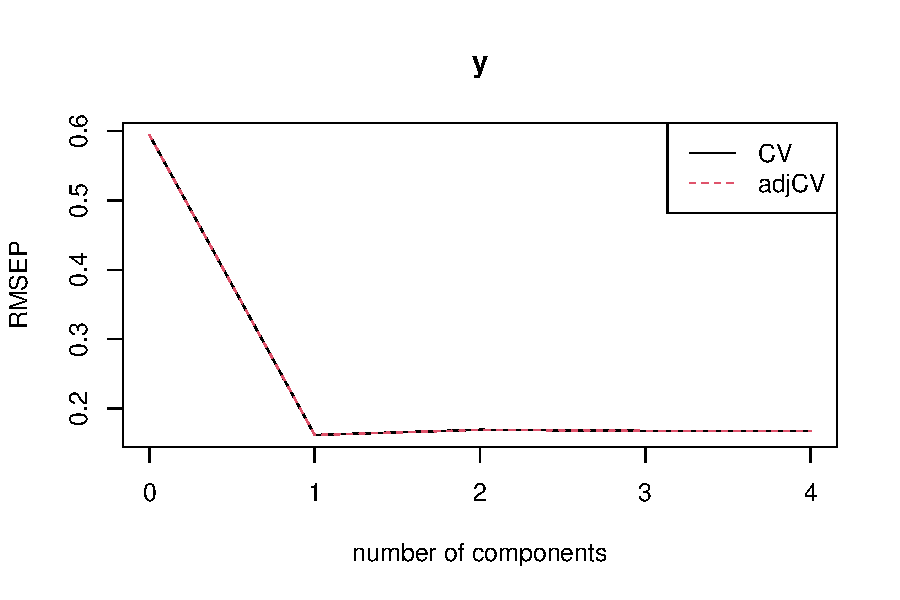
\includegraphics[width=12cm,height=10cm]{cv.pdf}
	\caption{CV for the number of components.}
	\label{fig:1}
\end{figure}
\newpage
\begin{figure}[h!]
	\centering
	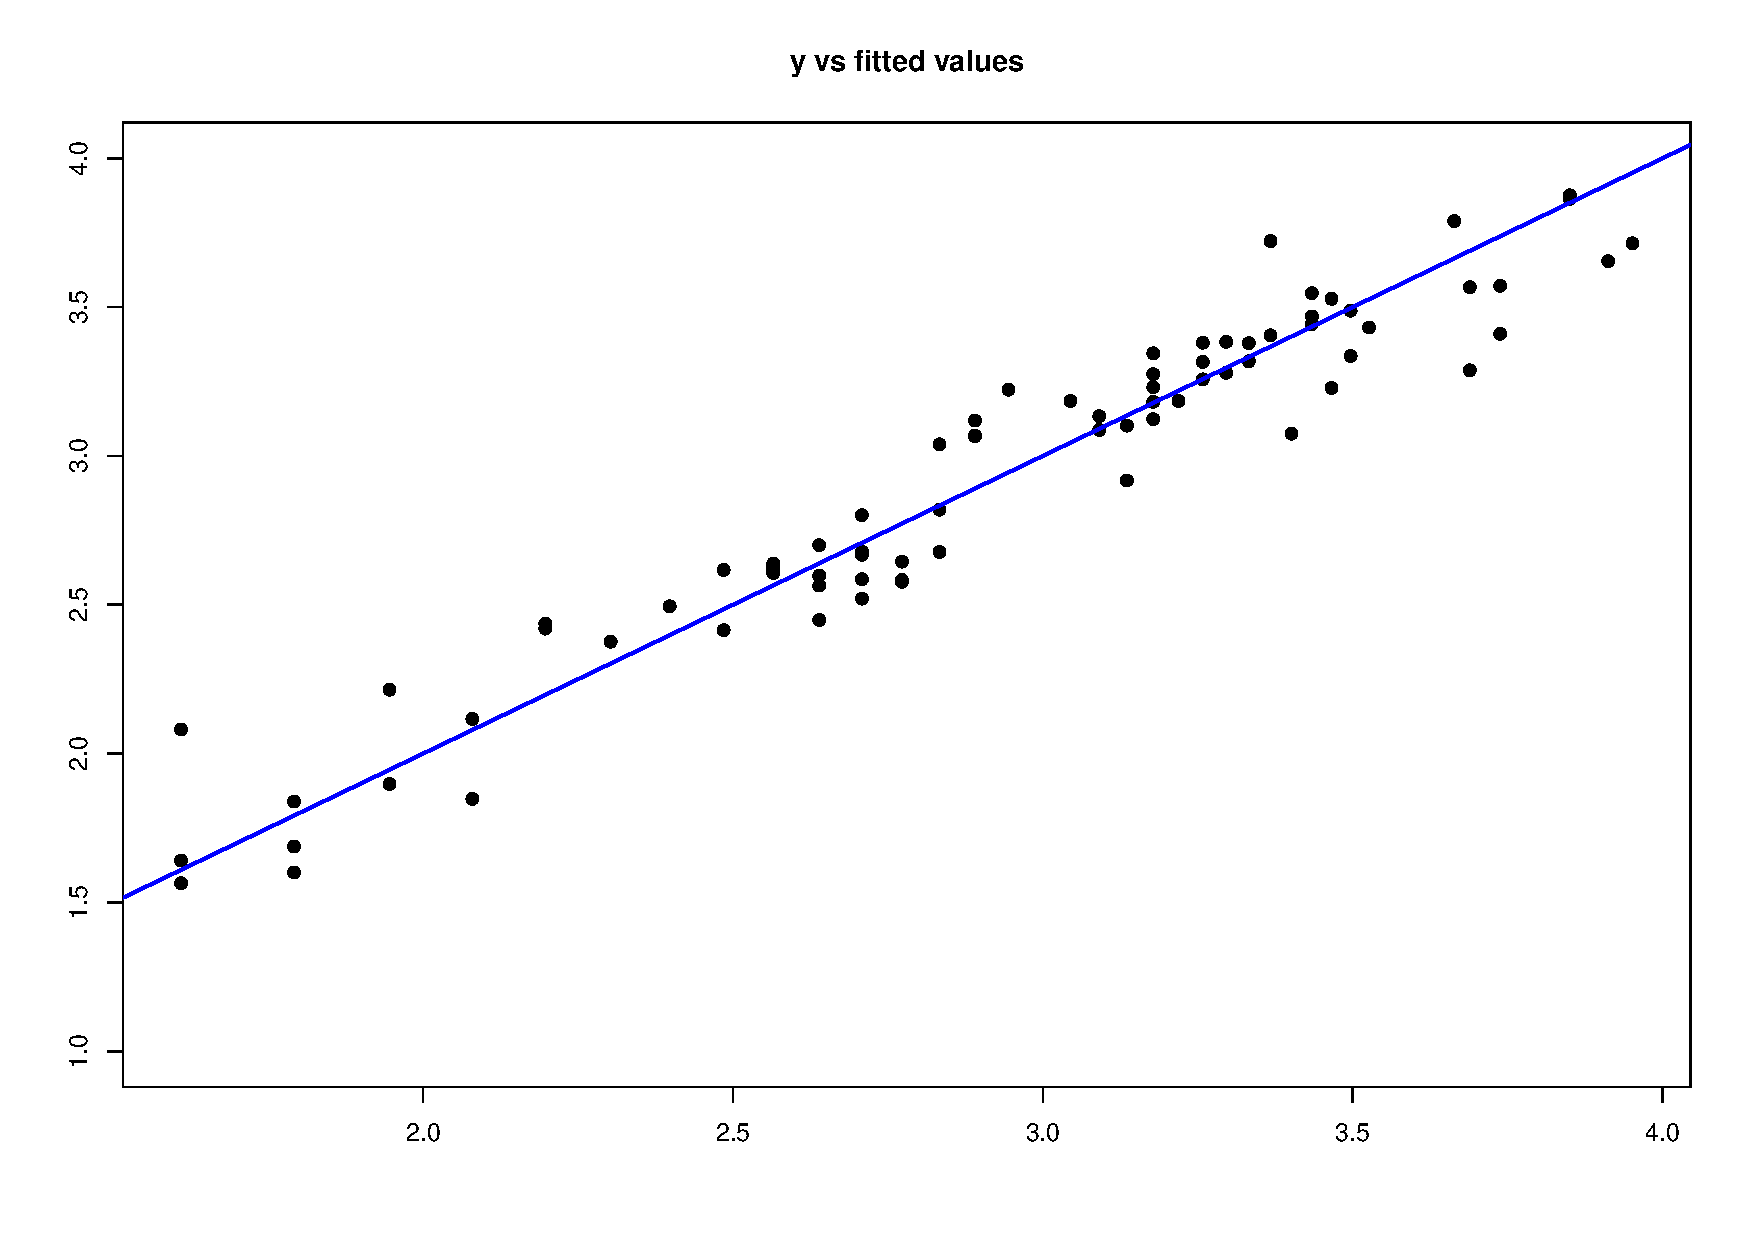
\includegraphics[width=16cm,height=14cm]{yvsfit.pdf}
	\caption{Plot for the response vector versus the fitted values for the PLS model $u=1$ along with the blue line that corresponds to $y=x$.}
	\label{fig:2}
\end{figure}
\newpage
\begin{figure}[h!]
	\centering
	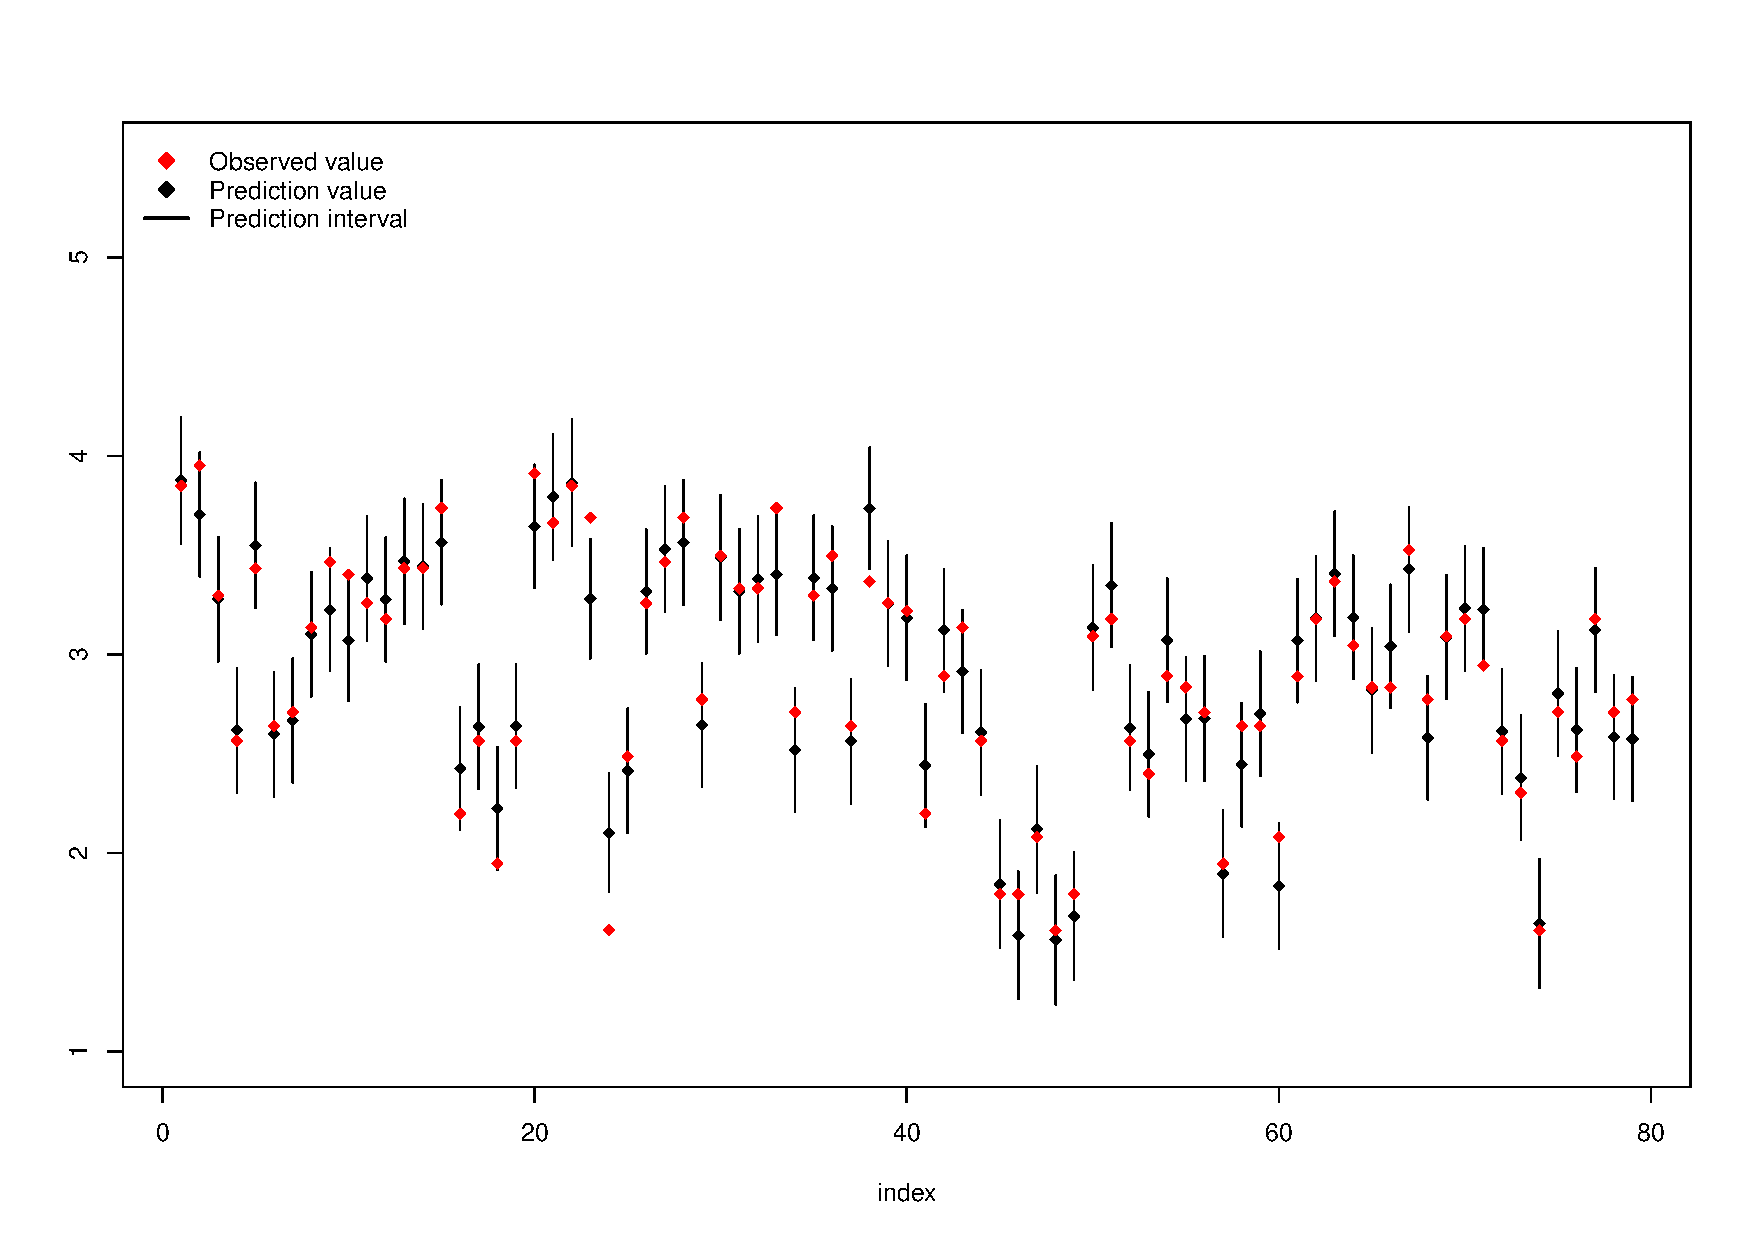
\includegraphics[width=18cm,height=14cm]{CImuss.pdf}
	\caption{Intervals for the $n=79$ observations in the mussels data. $93.67\%$ of the intervals contain the observed value.}
	\label{fig:3}
\end{figure}
\newpage
%Now we run the PLS fit with $u=1$ to obtain $\wbb_{pls} = (0.142,0.153,0.624,0.206)$. We can compare this with the estimated vector obtained in section $4.4.4.$ from \cite{c} (see Table 4.4), where $\wbb = (0.141,0.154,0.625,0.206)$.
Now we are going to compare the classic OLS estimation with PLS estimation. Furthermore, we also add the envelope estimation with $q=1$ obtained in section $4.4.4.$ from \cite{c}

\begin{table}[ht]
	\centering
	\caption{Results for the OLS regression}
	\begin{tabular}[t]{lccc}
		\hline
		&Value&Std & Confidence Interval \\
		$\widehat{\beta}_1$&$0.741$&$0.410$& $(-0.0759, 1.559)$\\
		$\widehat{\beta}_2$&$-0.113$&$0.399$& $(-0.909, 0.683)$\\
		$\widehat{\beta}_3$&$0.567$&$0.118$& $(0.330, 0.803)$\\
		$\widehat{\beta}_4$&$0.170$&$0.304$& $(-0.435, 0.776)$\\
		\hline
	\end{tabular}
\end{table}

\begin{table}[ht]
	\centering
	\caption{Results for the PLS regression with $u=1$}
	\begin{tabular}[t]{lccc}
		\hline
		&Value&Std & Confidence Interval \\
		$\widehat{\beta}_1$&$0.142$&$0.0063$& $(0.129, 0.154)$\\
		$\widehat{\beta}_2$&$0.153$&$0.0067$& $(0.140, 0.166)$\\
		$\widehat{\beta}_3$&$0.624$&$0.0199$& $(0.585, 0.663)$\\
		$\widehat{\beta}_4$&$0.206$&$0.0086$& $(0.189, 0.223)$\\
		\hline
	\end{tabular}
\end{table}

\begin{table}[ht]
	\centering
	\caption{Results for the envelope model, $q=1$}
	\begin{tabular}[t]{lccc}
		\hline
		&Value&Std & Confidence Interval \\
		$\widehat{\beta}_1$&$0.141$&$0.0052$& $(0.130, 0.151)$\\
		$\widehat{\beta}_2$&$0.154$&$0.0056$& $(0.143, 0.164)$\\
		$\widehat{\beta}_3$&$0.625$&$0.0194$& $(0.587, 0.663)$\\
		$\widehat{\beta}_4$&$0.206$&$0.0073$& $(0.191, 0.220)$\\
		\hline
	\end{tabular}
\end{table}

 We present here the four confidence intervals for $\widehat{\beta}_i$ for $i=1,2,3,4$ with these methods. Confidence intervals with PLS method were constructed following Corollary 2

\begin{equation*}
	\left[\wbb_{pls}^T \b{e}_i \pm z_{\alpha/2} \widehat{V}_{\b{e}_i}^{1/2} \right]
\end{equation*}
where $\b{e}_i$ is the vector with a $1$ in the $i$-th position and $0$'s elsewhere.

\begin{figure}[h!]
	\centering
	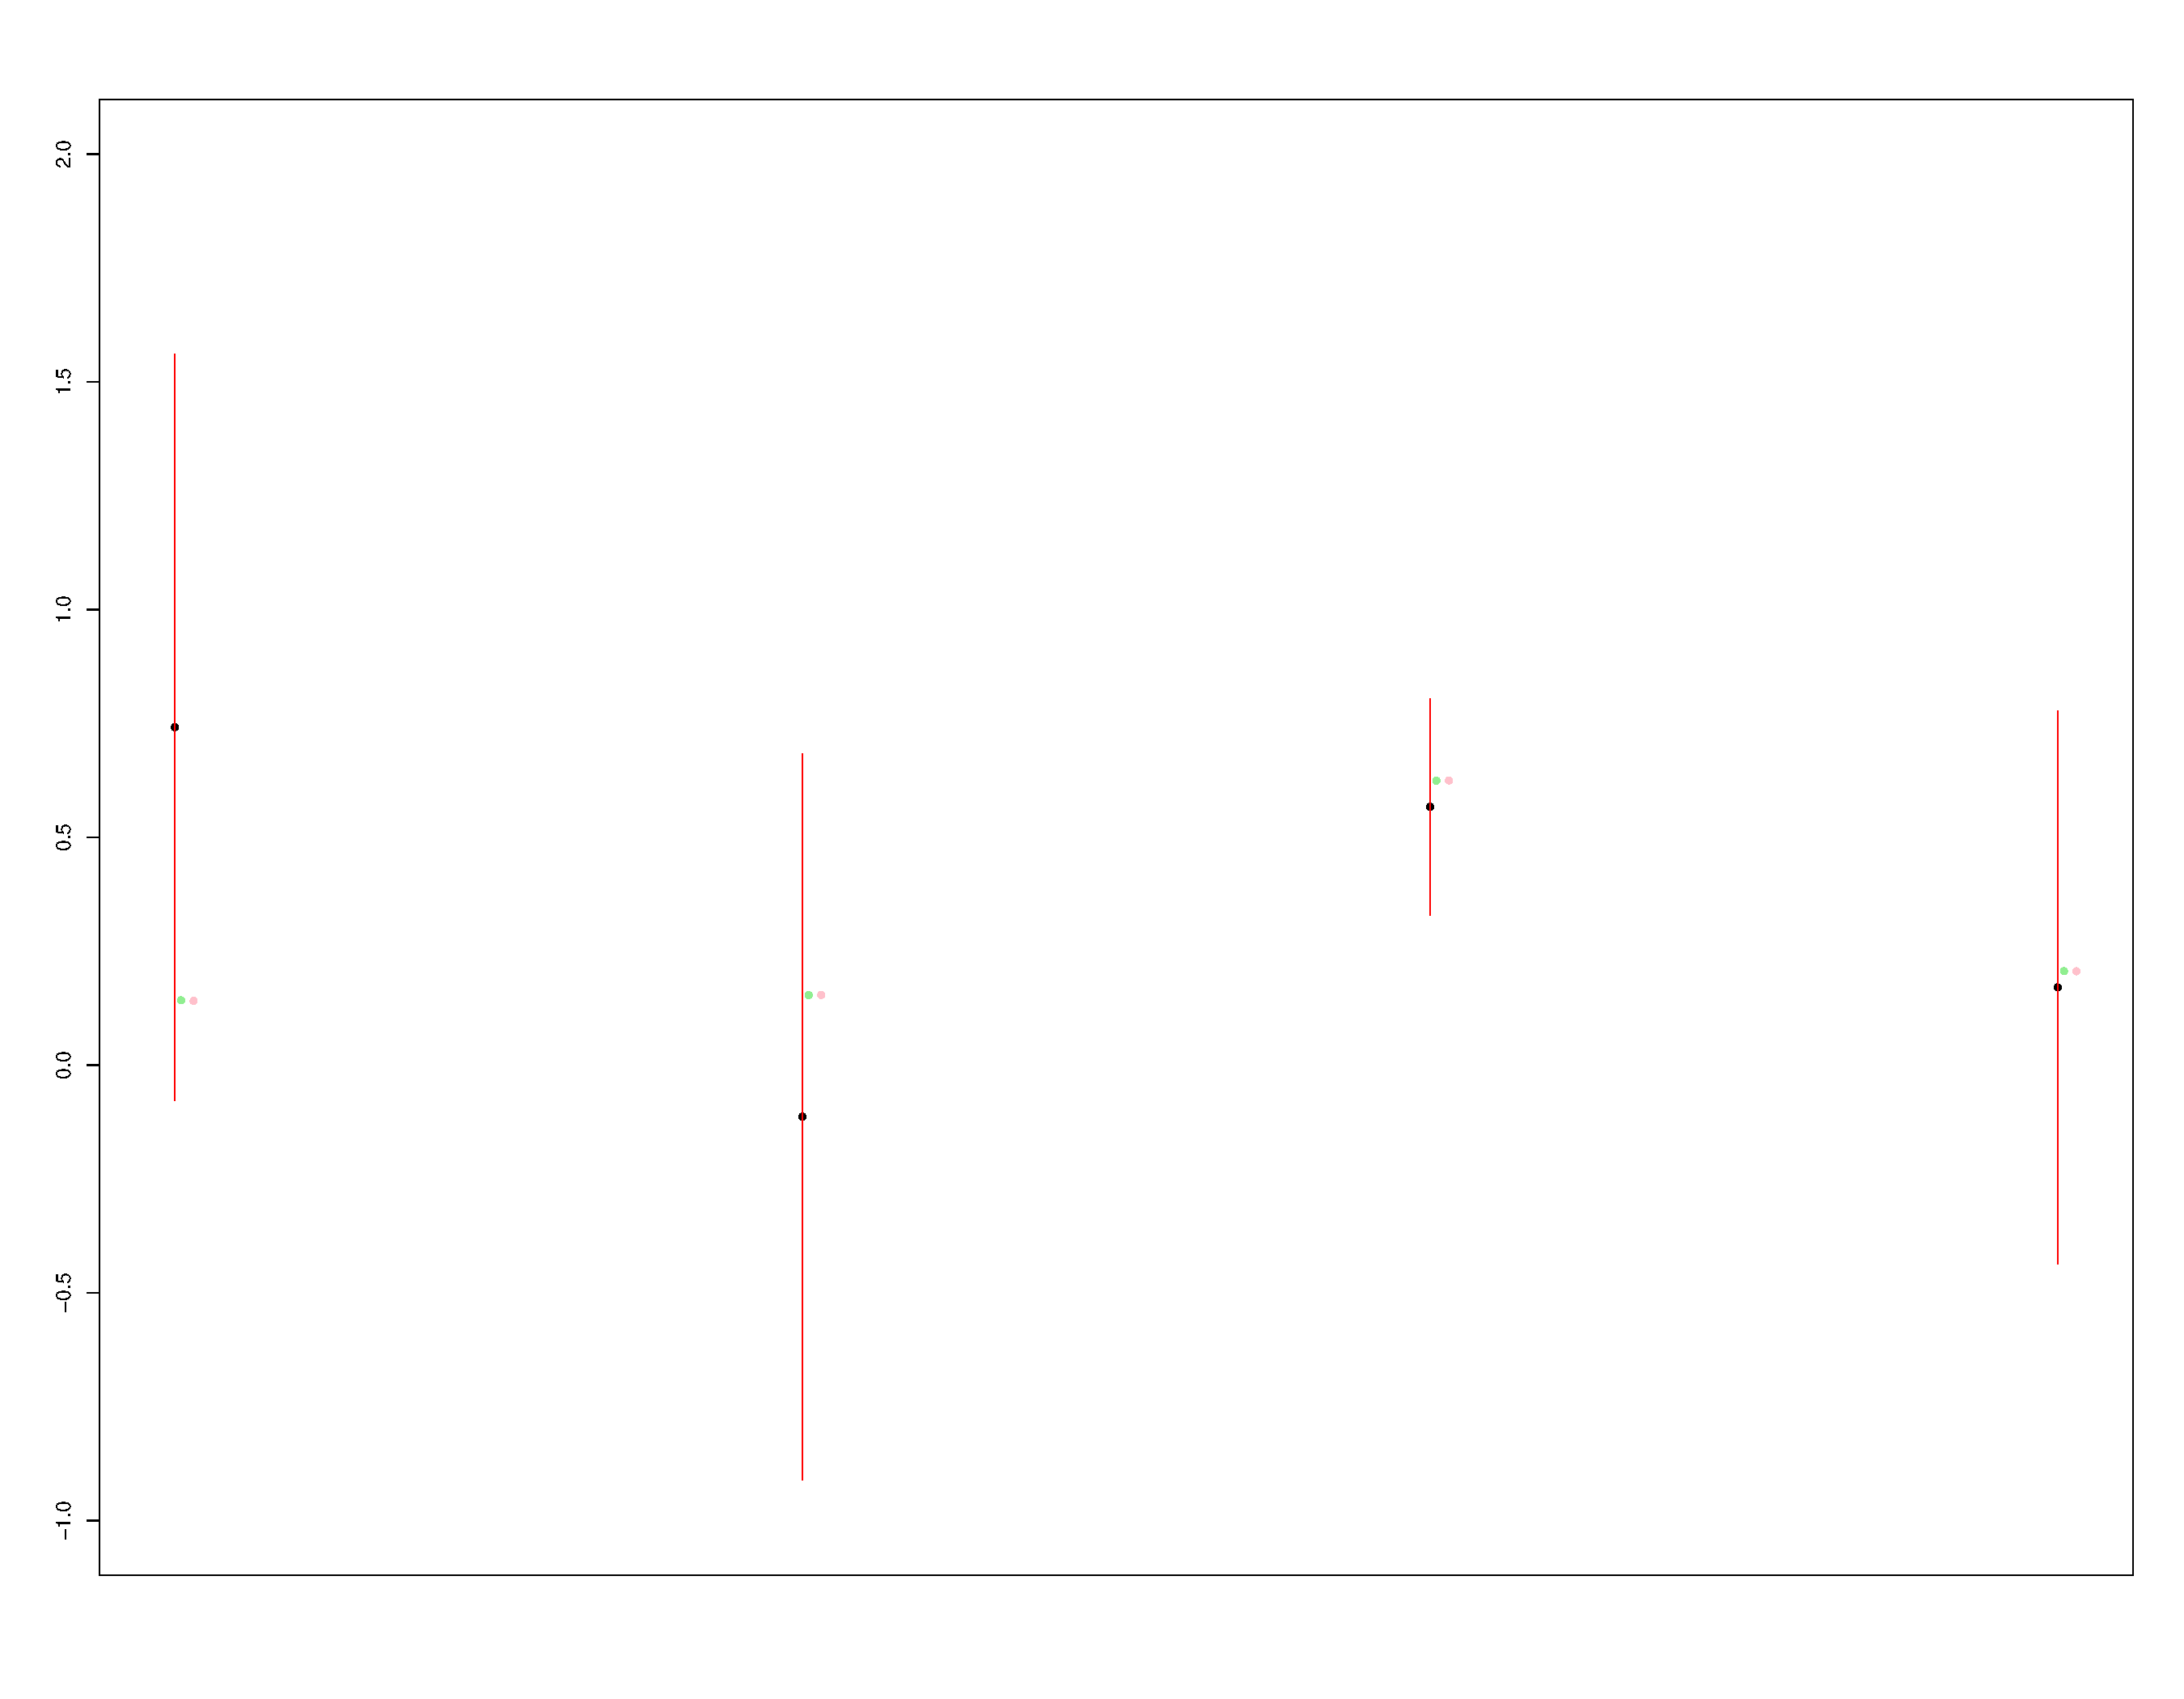
\includegraphics[width=18cm,height=14cm]{CIbetas.pdf}
	\caption{Comparison between the OLS, PLS and envelope estimations for $\widehat{\beta}_i$ for $i=1,2,3,4$. Observe that while the intervals for PLS and envelopes are quite similar, the intervals for OLS are significantly greater.}
	\label{fig:4}
\end{figure}
\newpage
\begin{thebibliography}{9}
\bibitem{c}
Cook, R. D., \textit{An Introduction to Envelopes: Dimension Reduction for Efficient Estimation in Multivariate Statistics}, Wiley Series in Probability and Statistics, ISBN = 9781119422969
\end{thebibliography}



\end{document}